%----------- Pin style
\tikzstyle{every pin edge}=[<-,shorten <=1pt]

%----------- Block style 1
\tikzstyle{neuron}=[circle,fill=black!25,minimum size=17pt,inner sep=0pt]

%----------- Block style 1
\tikzstyle{input neuron}=[neuron, fill=green!50]

%----------- Block style 1
\tikzstyle{output neuron}=[neuron, fill=red!50]

%----------- Block style 1
\tikzstyle{hidden neuron}=[neuron, fill=blue!50]

%----------- Block style 1
\tikzstyle{annot} = [text width=4em, text centered]

% Define a distance to separate the layers of the network
\def\layersep{2.5cm}

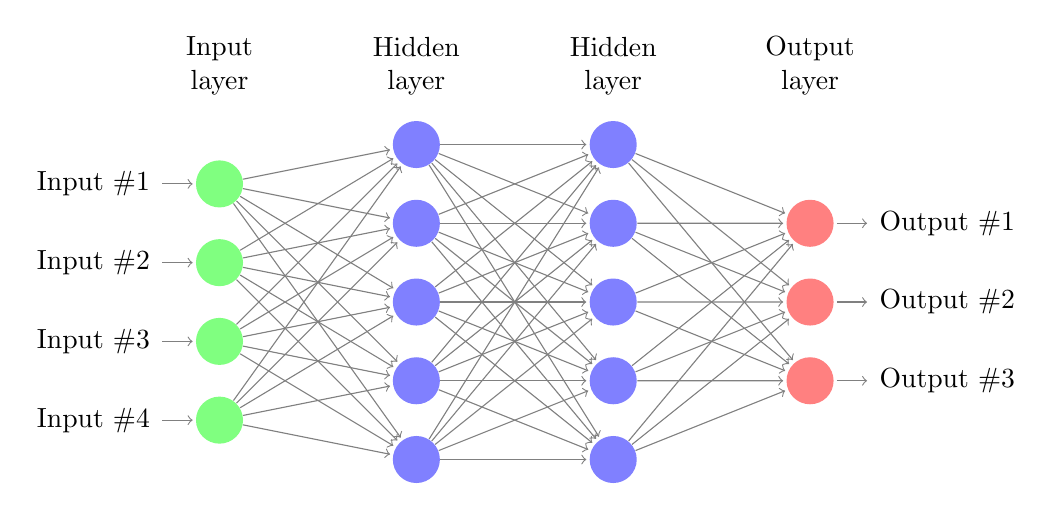
\begin{tikzpicture}[shorten >=1pt,->,draw=black!50, node distance=\layersep]
    
    % Draw the input layer nodes
    \foreach \name / \y in {1,...,4}
    % This is the same as writing \foreach \name / \y in {1/1,2/2,3/3,4/4}
        \node[input neuron, pin=left:Input \#\y] (I-\name) at (0,-\y) {};

    % Draw the hidden layer 1 nodes
    \foreach \name / \y in {1,...,5}
        \path[yshift=0.5cm]
            node[hidden neuron] (H1-\name) at (\layersep,-\y cm) {};
	
	% Draw the hidden layer 2 nodes
	\foreach \name / \y in {1,...,5}
		\path[yshift=0.5cm]
			node[hidden neuron] (H2-\name) at (2*\layersep,-\y cm) {};
	
    % Draw the output layer node
    \foreach \name / \y in {1,...,3}
    	\path[yshift=-0.5cm]
    		node[output neuron, pin={[pin edge={->}]right:Output \#\y}] (O-\name) at (3*\layersep,-\y cm) {};

    % Connect every node in the input layer with every node in the
    % hidden layer 1.
    \foreach \source in {1,...,4}
        \foreach \dest in {1,...,5}
            \path (I-\source) edge (H1-\dest);
	
	% Connect every node in hidden layer 1 with every node in
	% hidden layer 2.
	\foreach \source in {1,...,5}
		\foreach \dest in {1,...,5}
			\path (H1-\source) edge (H2-\dest);
	
    % Connect every node in the hidden layer with the output layer
    \foreach \source in {1,...,5}
    	\foreach \dest in {1,...,3}
        	\path (H2-\source) edge (O-\dest);

    % Annotate the layers
    \node[annot,above of=H1-1, node distance=1cm] (h1) {Hidden layer};
    \node[annot,above of=H2-1, node distance=1cm] (h2) {Hidden layer};
    \node[annot,left of=h1] {Input layer};
    \node[annot,right of=h2] {Output layer};
    
\end{tikzpicture}